\documentclass[../main.tex]{subfiles}

\begin{document}
Für dieses Projekt wird das Entwicklungsprogram Unity und seine Physics Engine eingesetzt. Das Script für die physikalischen Vorgänge wird in C Sharp geschrieben.

\subsection{Lab 2: Würfel bewegt sich und stösst}
Als Grundgerüst ist die Szene vom ersten Lab übernommen worden und der Aufgabenstellung ergänzt. Alle Kräfte und Berechnungen befinden sich im Skript CubeController.cs, welches im Anhang [ref] ersichtlich ist. Zur Kontrolle der Werte und Grafik Erstellung werden zwei verschiedene CSV Datei erstellt (timeseries genannt), eine für den elastischen Stoss relevanten Werte und eine für den inelastischen Stoss.

    \begin{figure}[H]
        \begin{center}
        \centerline{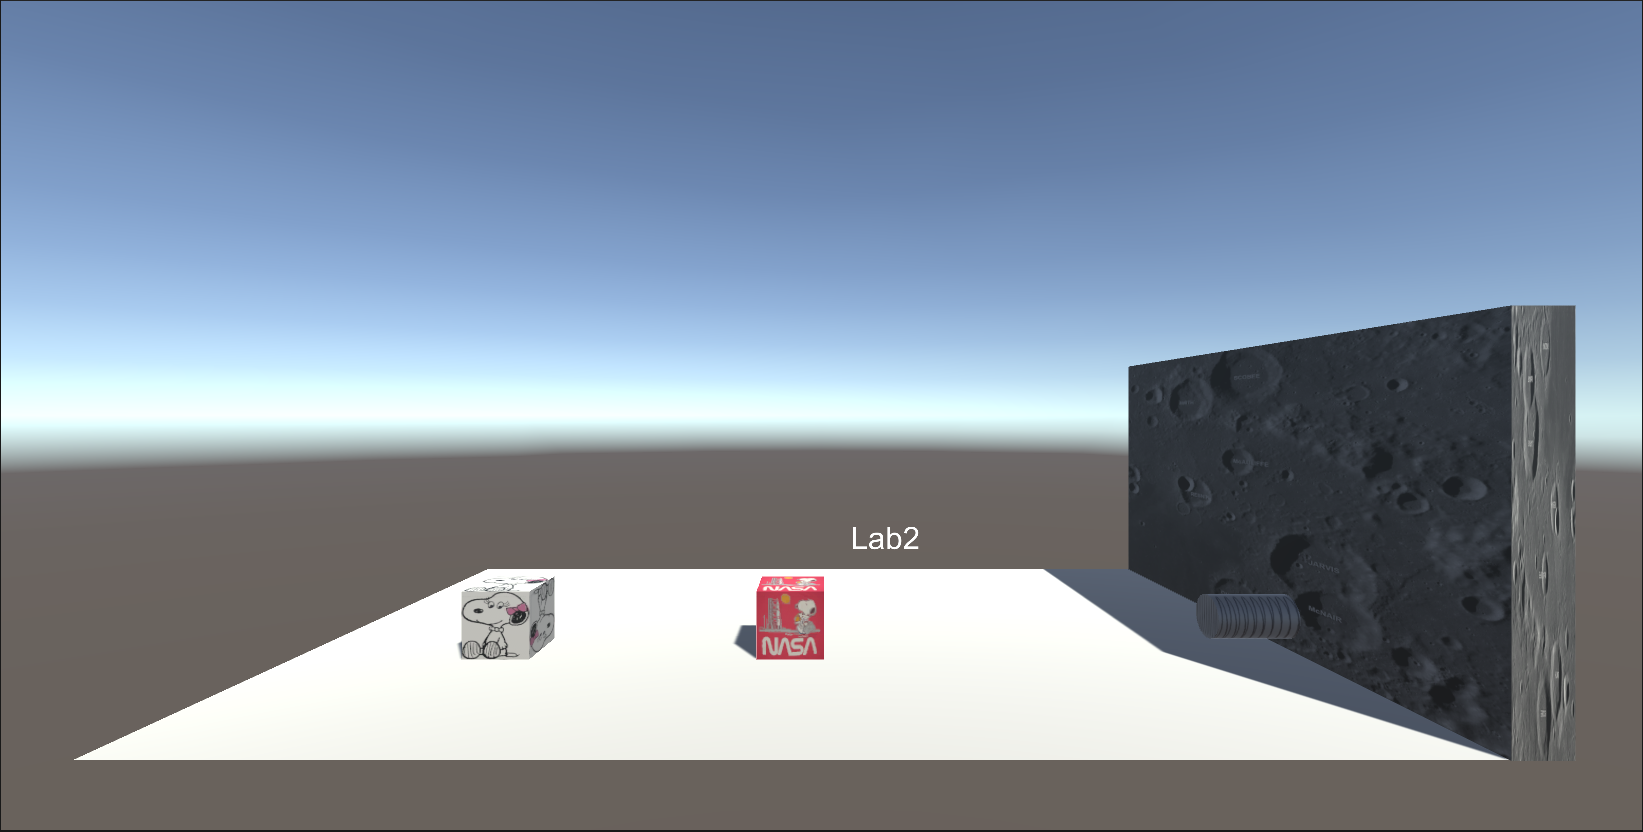
\includegraphics[width=155mm]{./images/2Lab_ExperimentOverview}}
            \caption{Experiment Übersicht}
            \label{fig:2Lab_ExperimentOverview}
        \end{center}
    \end{figure}

Folgend sind einige wichtige Eigenschaften der Lab relevanten Objekte in Unity:

\begin{itemize}
    \item Julia:
    \newline Für die Seitenlänge ist die Scale auf 1.5 angepasst, da in Unity beim Würfel eine Seitenlänge von 1 besitz. Somit entspricht beim Würfel die Seite jeweils dem Scale Wert. Wichtig ist nicht zu vergessen, das Material auf reibungslos zu ändern, sonst bewegen sich die Würfel nicht richtig.
    \begin{figure}[H]
        \begin{center}
        \centerline{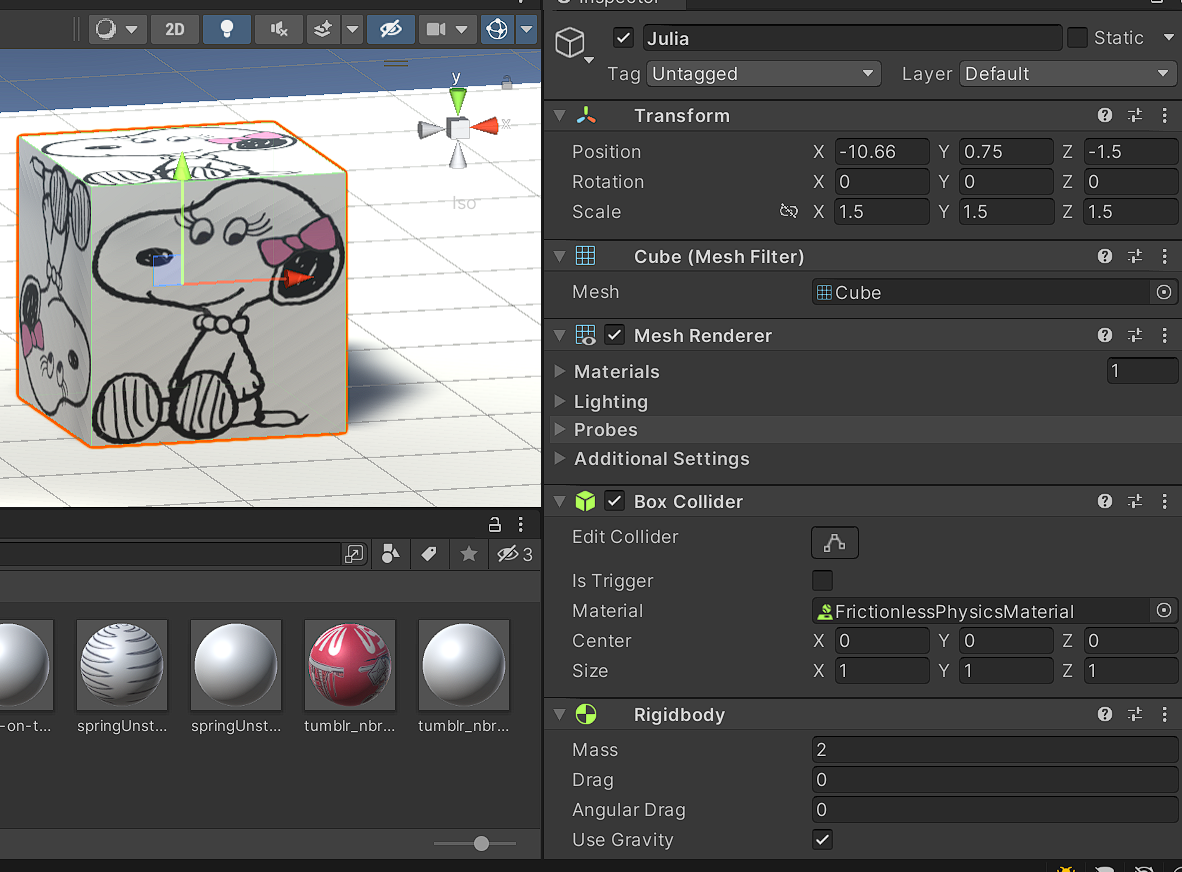
\includegraphics[width=100mm]{./images/2Lab_JuliaCube.PNG}}
            \caption{Einstellung Julia}
            \label{fig:2Lab_JuliaCube}
        \end{center}
    \end{figure}

    \item Romeo: 
    \newline Die Eigenschaften sind ausser der Position und Farbe gleich wie Julia. Zusätzlich ist hier das Skript angehängt. Damit das Skript auf die Objekte richitg referenzieren kann, werden sie hier als Variabel mitgegeben.
    \begin{figure}[H]
        \begin{center}
        \centerline{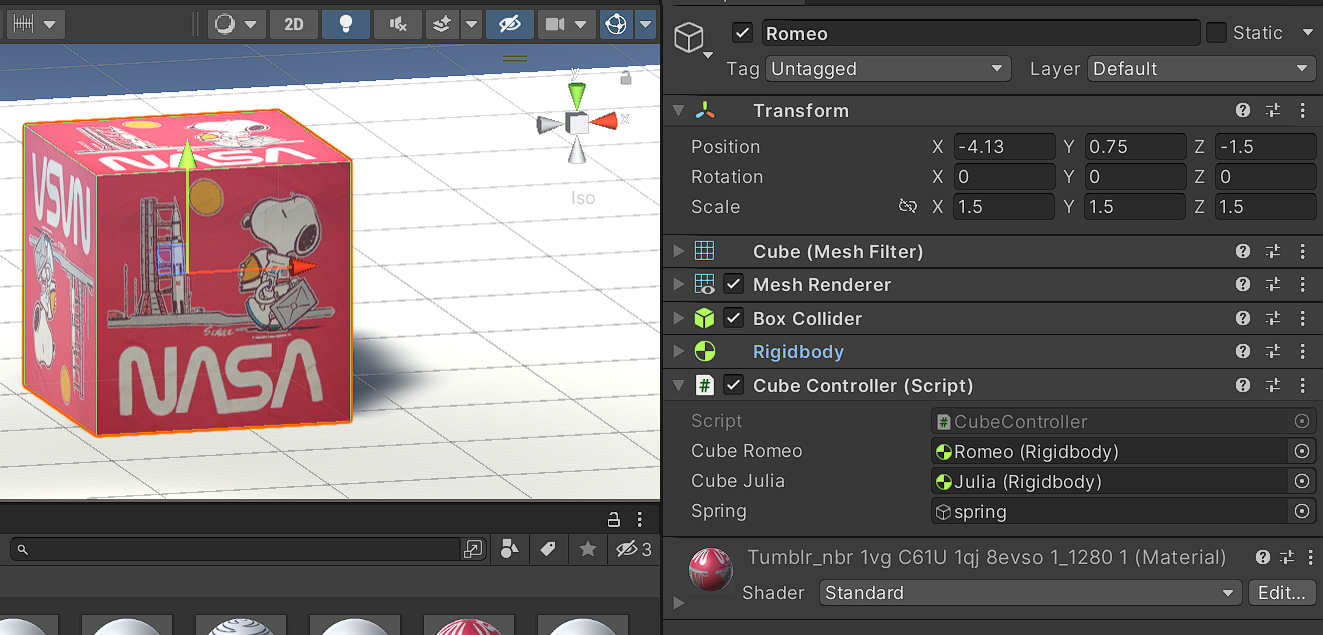
\includegraphics[width=100mm]{./images/2Lab_RomeoCube.PNG}}
            \caption{Einstellung Romeo}
            \label{fig:2Lab_RomeoCube}
        \end{center}
    \end{figure}

    \item Spring:
    \newline Wie in Abbildung \ref{fig:2Lab_RomeoCube} zu sehen ist die Feder nur als GameObject und nicht als Rigdbody im Skript angegeben. Die Ausrichtung wurde entlang der Y-Achse belassen und um 90 Grad rotiert damit der Zylinder liegend erscheint.
    \begin{itemize}
        \item Mesh: Cylinder
        \item Collider direction: Y-Axis
        \begin{figure}[H]
            \begin{center}
            \centerline{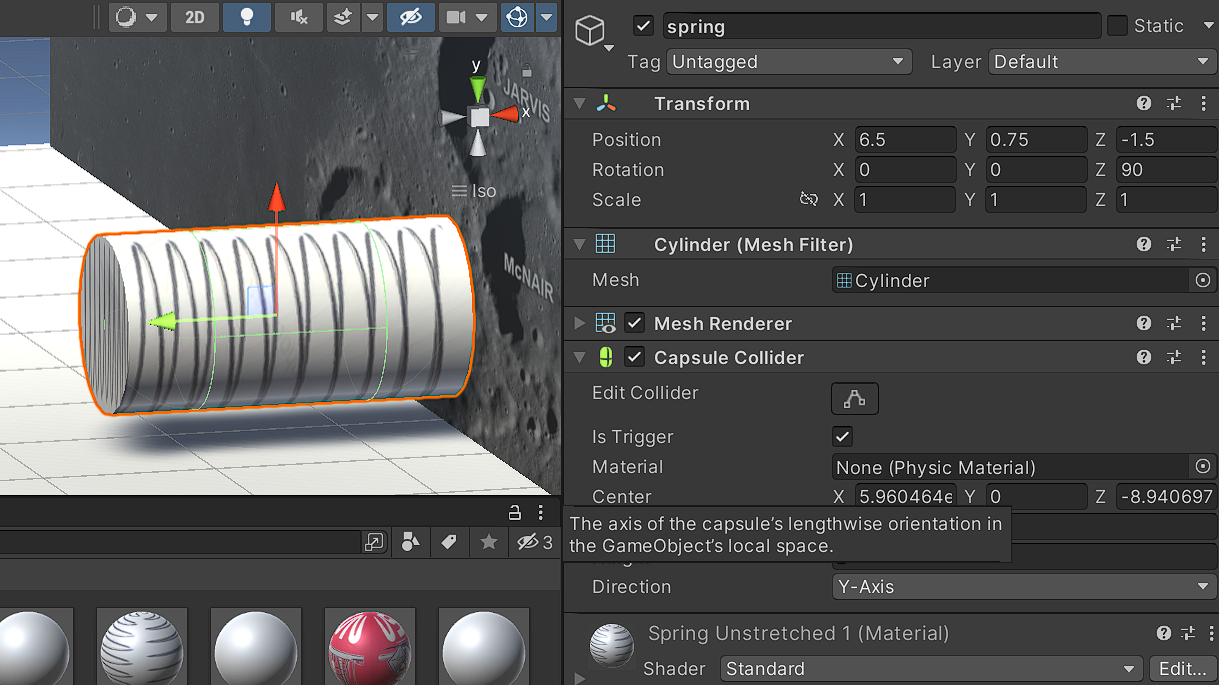
\includegraphics[width=100mm]{./images/2Lab_Spring.PNG}}
                \caption{Einstellung Feder}
                \label{fig:2Lab_Spring}
            \end{center}
        \end{figure}
    \end{itemize}

    \item Plane
    \begin{itemize}
        \item Collider Material: FrictionlessPhysicsMaterial
    \end{itemize}
\end{itemize}

\newpage
Da es  sich beim CubeController um ein Unity Skript handelt, wird von der Klasse Monobeviour geerbt, damit methoden wie FixedUpdate oder OnCollisionEnter benutzt werden kann.

Im Code wird am Anfang die konstate Kraft (constantForce) mit 4 und die Beschleunigunszeit (accelarationTime) mit 1 festgelegt, wie im Kapitel 3.1.1 Konstante Kraft [ref] berechnet. Für die Federauslenkung wird 1.5 gewählt, da die Feder eine Länge von 2 hat und vorher gestoppt werden muss bevor Romeo auf die Wand auftrifft.

In der Start Methode wird aus den gegebenen Werten die Federkonstante berechnet.
\begin{lstinputlisting}[label={lst:graphInelastic}, firstline=50, lastline=51]
    {..//UnityProj/Assets/CubeController.cs}
    \end{lstinputlisting}

Es wird auch die Position gespeichert, welche Romeo zum ersten Mal die Feder auftrifft (springMaxDeviation) wie in Abbildung \ref{fig:2Lab_SpringDeviation} rot markiert. 
\begin{lstinputlisting}[label={lst:graphInelastic}, firstline=46, lastline=49]
    {..//UnityProj/Assets/CubeController.cs}
    \end{lstinputlisting}


\begin{figure}[H]
    \begin{center}
    \centerline{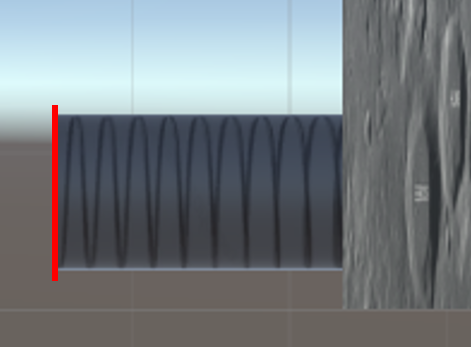
\includegraphics[width=50mm]{./images/2Lab_SpringDeviation.PNG}}
        \caption{Einstellung Feder}
        \label{fig:2Lab_SpringDeviation}
    \end{center}
\end{figure}

Danach werden die Timeseries Listen deklariert, für die CSV Dateien. Das Hinzufügen der Werte passiert kontinuierlich in der Methode FixedUpdate.
\newline 
In FixedUpdate gibt es zwei If-Bedingungen. Die erste ist zum Hinzufügen der oben erwähnte constantForce mit der Methode .AddForce bis die Beschleunigunszeit vorüber ist. 

Die zweite If-Bedingung ist zur Überprüfung, ob Romeo die Feder berührt. Dafür muss die Position der rechten Kante von Romeo ausgerechnet werden. mit der springMaxDeviation verglichen werden. 

Im Code wird der Würfel, welcher am Anfang beschleunigt wird, Romeo benannt und der andere Würfel entsprechend
Julia. Die Würfel werden in den nächsten Abschnitten ebenfalls so bezeichnet, damit man denn Zusammenhang mit den
Screenshots des Codes leichter versteht. Zur Kontrolle der Werte und Grafik Erstellung wurde zwei verschiedene
CSV Datei erstellt (timeseries genannt), eine für den elastischen Stoss relevanten Werte und eine für den inelastischen Stoss.
\newline
Für die Beschleunigung von Romeo wird gemäss Berechnung, eine konstante Kraft von 4 (Newton) im FixedUpdate hinzugefügt.
Die Beschleunigunszeit von einer Sekunde wird von den Autoren bestimmt.
Der Würfel braucht also eine Sekunde um die maximale Geschwindigkeit zu erreichen.
Die konstante Kraft wirkt solange bis die Geschwindigkeit von 2m/s erreicht.
Dabei wird Romeo wird dann auch die kinetische Energie berechnet und in beiden Timeseries notiert.
\newline
Beim Teil mit dem elastischen Stoss wurde ein Feder GameObject hinzugefügt. Die Federkonstante wird am Start berechnet
bevor sich Romeo bewegt. Dies wird wie in der Berechnung erwähnt das Energieerhaltungsgesetz angewendet und für die
Federstauchung wurde 1.3 (Meter) gewählt, sodass der berechnete Federkonstante Wert 4.733 (N/m) beträgt. Beim Start
wird ebenfalls die Position der Feder in der Ruhelage, dort welche Romeo die Feder zuerst berühren würde, in der
Variable springMaxDeviation gespeichert.
\newline
Diese wird in FixedUpdate gebraucht um zu überprüfen, ob Romeo bereits auf die Feder eintrifft.
Sobald dies der Fall ist, verändert sich die Texture von Romeo und dann wird jeweils die Federkraft darin
berechnet und an Romeo hinzugefügt. Dafür wird der Längenunterschied der Feder mit der Differenz aus der
Position von Romeo und springMaxDeviation berechnet und danach mit der negativen Federkonstante multipliziert.
Dadurch bewegt sich Romeo  zurückt. Als Überprüfung der Energieerhaltung wird schlussendlich auch die potentiele
Energie der Feder berechnet und in der elastischen Timeseries zusammen mit der Federkraft aufgeschrieben.
\newline
Für den inelastischen Stoss mit Julia wird im OnCollisionEnter jeweils geprüft, ob es sich bei der Kollision um
Julia handelt. Nur wenn dies der Fall ist, wird dann ein FixedJoint an den Berührungspunkte zwischen Romeo und
Julia hinzugefügt um die damit sie zusammenkleben. Zum Schluss muss noch .enableCollision auf false gesetzt werden,
damit sich die beiden Würfeln nicht mehr kollidieren.
\newline
Im FixedUpdate wird dann für die inelastische Timeseries die Impulse berechnet und die gemeinsame Endgeschwindigkeit
und kinetische Energie. Mit dieser Geschwindigkeit kann dann auch die Kraft welche auf Julia wirkt errechnet werden.


    @kimmie: pls descibe
    - script in c#
    - klass erbt monobehavior
    --> bietet riged body, on bxo collieder, alle methoden die gebraucht werden
    - einezlne objekte
    - inelastisch fixejoint (screenshot)
    - erklärung warum spring gameobject und nicht rigedbody
    - screenshots von unity mit guggus infos :D
    - wenn uf code willsch iga:


  code uf bestimmti ziele:
    \begin{lstinputlisting}[label={lst:graphInelastic}, firstline=7, lastline=12]
    {..//UnityProj/Assets/CubeController.cs}
    \end{lstinputlisting}

    \begin{itemize}
        \item Julia:
        \begin{itemize}
            \item Material
            \item Cube
            \item Boxcolider enabled
            \item Contraints
            \item Frictionless
        \end{itemize}

        \item \item Romeo:
        \begin{itemize}
            \item Wall
            \item Lame
            \item Süffel
        \end{itemize}
    \end{itemize}

\end{document}